\documentclass[pdflatex,sn-basic]{sn-jnl}

\usepackage{graphicx}
\usepackage{booktabs}
\usepackage{amsmath,amssymb,amsfonts}
\usepackage{amsthm}
\usepackage{xcolor}
\usepackage{textcomp}
\usepackage{manyfoot}
\usepackage{listings}
\usepackage{xspace}
\hypersetup{
  pdftitle={SafeMAP: Analysis-Guided Planning and Per-Function Validation for Safe C-to-Rust Translation},
  pdfauthor={Jacob Sebastian Cyril; Benita Jose Chalissery; NewBegin M},
  pdfkeywords={C-to-Rust migration, safe Rust, static analysis, large language models, differential testing, memory safety}
}

\newcommand{\tool}{SafeMAP\xspace}
\newif\ifanonymous
\anonymousfalse % Change only if the eventual venue requires anonymous review.

\begin{document}

\title[SafeMAP: Analysis-Guided Planning and Per-Function Validation]{SafeMAP: Analysis-Guided Planning and Per-Function Validation for Safe C-to-Rust Translation}

\ifanonymous
\author*[1]{\fnm{Anonymous} \sur{Submission}}
\else
\author*[1]{\fnm{Jacob Sebastian} \sur{Cyril}}\email{jacob.sebastian@mca.christuniversity.in}
\author[1]{\fnm{Benita Jose} \sur{Chalissery}}\email{benita.jaison@christuniversity.in}
\author[1]{\fnm{NewBegin} \sur{M}}\email{new.begin@christuniversity.in}
\fi

\affil*[1]{\orgdiv{Department of Computer Science}, \orgname{CHRIST (Deemed to be) University}, \orgaddress{\city{Bangalore}, \country{India}}}

\abstract{Automatic C-to-Rust translators either keep C's pointer conventions
in unsafe Rust or rely on a large language model (LLM) whose output is hard to
check. \tool is a conservative alternative. For each C function it first
decides, by static analysis, whether a safe Rust interface exists; if not, it
refuses the function and records why. For the remaining functions it emits
Rust from exact rules or from a plan-guided LLM request with compiler-feedback
repair, and it accepts a function only if the code contains no
\texttt{unsafe}, exposes no raw pointers, and matches the original C function
on up to 1,000 generated inputs, with the C side run under AddressSanitizer
and UndefinedBehaviorSanitizer. We froze the implementation and evaluated it
on ten held-out C libraries (9,456 lines, 356 translation units) selected by
a sealed protocol. Across three runs, \tool accepted 12--16 units and a
one-shot LLM given the same planned interfaces 9--15; rules alone accepted 1
and raw C2Rust none.
Most units were refused before translation: 159 need manual refactoring and
116 use C types with no safe, testable Rust interface. Mutation analysis shows
that the per-function check rejects 89\% of compiling single-operator mutants
of accepted functions. Ablations on development libraries attribute the
accepted translations mainly to safe-signature planning and idiom plans, not
to prompt guidance or repair; with the planned interfaces, a single LLM request
performs within the run-to-run range of the full loop. The results show that per-function,
oracle-checked acceptance is feasible on production C but that coverage is
low; the recorded refusals identify what currently blocks automatic safe
migration.}

\keywords{C-to-Rust migration, safe Rust, static analysis, large language
models, differential testing, memory safety}

\maketitle

\section{Introduction}

C remains common in systems software. Its memory model leaves programmers
responsible for preventing buffer overflows, use-after-free errors, null
dereferences, and data races. Safe Rust checks ownership and borrowing at
compile time while retaining low-level control, so migrating C code to safe
Rust is attractive. Translation is difficult because many C idioms have no
direct safe-Rust equivalent: raw pointers, output parameters, manual
allocation, nullable values, and integer error codes all require changes in
representation and interface.

C2Rust preserves C behavior by generating Rust that uses raw pointers and
unsafe operations \cite{c2rust}. Later work reduces this unsafety by static
analysis, ownership inference, refactoring, and LLM rewriting
\cite{emre2021safer,hong2023static,zhang2023ownership,ling2022trust,
nitin2026c2saferrust,mohapatra2026cp2srust}. A second line asks LLMs to
translate directly to safe Rust and checks the result with tests, fuzzing, or
verification
\cite{hong2025typemigrating,zhou2025c2rusttv,eniser2025fluorine,
shetty2024syzygy,zhou2025sactor,yang2025vert,sim2026encrust}. These systems
generally aim to translate everything and then measure how much of the result
is safe or correct.

\tool takes the opposite position. It translates a function only when static
analysis finds a safe Rust interface for it, and it accepts a translation only
when that function, on its own, passes a behavioral check against the
original C. Everything else is refused with a recorded reason. The question
is therefore not how much unsafe code remains, but how many functions of real
C code can be migrated to safe Rust with per-function evidence, and what
prevents the rest.

An earlier, frozen evaluation of \tool on three C libraries accepted no
units: defects in interface planning, rule matching, and harness construction
each forced the outcome to zero (Section~\ref{sec:history}). This paper
reports the corrected system, evaluated under a new sealed protocol on ten
libraries that were not used during development. We ask:

\begin{itemize}
  \item \textbf{RQ1:} How many translation units of production C libraries
  does \tool accept as safe, behaviorally validated Rust?
  \item \textbf{RQ2:} Why are the remaining units not accepted?
  \item \textbf{RQ3:} How does \tool compare with a one-shot LLM given the
  same interfaces, with its own rules alone, and with raw C2Rust, under one
  acceptance policy?
  \item \textbf{RQ4:} Which planning components contribute to acceptance?
  \item \textbf{RQ5:} How reliable is the acceptance decision, in terms of
  the harness's ability to reject wrong code and the variation across LLM
  runs?
\end{itemize}

This paper contributes:

\begin{itemize}
  \item a translation pipeline that decides, per function and before any
  translation, whether a safe and testable Rust interface exists, and records
  a reason when it does not;
  \item a per-function acceptance procedure that compares each Rust function
  with the original C function under sanitizers, excluding inputs on which the
  C code has undefined behavior;
  \item a sealed, frozen evaluation on ten held-out libraries with a one-shot
  LLM baseline that receives the same interfaces, repeated LLM runs, mutation
  analysis of the acceptance check, and component ablations; and
  \item a breakdown of 356 held-out units by the reason they could not be
  migrated, together with a public artifact for every decision.
\end{itemize}

\section{Background and related work}

\subsection{C2Rust and safer-Rust refactoring}

C2Rust translates C through a mostly syntactic process and is often used as a
baseline or a migration starting point \cite{c2rust}. It preserves many C
constructs with raw pointers and unsafe operations, so much of its output falls
outside Rust's safe subset. Emre et al.\ found that raw pointers cause much of
this unsafety \cite{emre2021safer}. Hong used static analysis to replace
selected unsafe constructs in C2Rust output, including lock APIs and output
parameters \cite{hong2023static}. C2SaferRust combines C2Rust, static
analysis, and LLM rewriting to reduce unsafe code in translated real-world
programs \cite{nitin2026c2saferrust}. Crown infers ownership models for C
pointers and converts many of them to safe Rust types
\cite{zhang2023ownership}. CRustS and Cp2SRust use different source-to-source
transformations and transpiler designs
\cite{ling2022trust,mohapatra2026cp2srust}. Industry studies and surveys report
that automatic translation still needs substantial manual work and testing
\cite{hong2025cacm,viirola2026feasible}.

\subsection{LLM-based C-to-Rust translation}

LLMs can produce idiomatic Rust, although correctness and type migration remain
open problems. Hong and Ryu studied an LLM translator supplied with candidate
signatures, caller and callee context, and compiler feedback
\cite{hong2025typemigrating}. C2RustTV checks LLM translations with generated
tests and repair loops \cite{zhou2025c2rusttv}. Eniser et al.\ evaluate LLM
translation through cross-language differential fuzzing and find lower success
on more complex real-world samples \cite{eniser2025fluorine}. RustFlow studies
prompting and iterative repair \cite{zhang2026rustflow}. Valenzuela et al.\
examine compiler errors in direct C-to-safe-Rust translation
\cite{valenzuela2026llmcompile}. RustMap combines program analysis and LLM
support at project scale \cite{cai2025rustmap}.

Several recent systems validate LLM translations against the C program.
Syzygy translates units in dependency order and tests each one against its C
counterpart with LLM-generated inputs \cite{shetty2024syzygy}. SACTOR first
produces interface-preserving Rust that may use \texttt{unsafe}, then refines
it to idiomatic safe Rust, and checks both stages with end-to-end tests linked
to the C code through the foreign-function interface \cite{zhou2025sactor}.
VERT checks a readable LLM translation against a WebAssembly-derived oracle
with bounded model checking or property-based testing \cite{yang2025vert}.
ENCRUST wraps LLM translations in ABI-preserving shims and removes the
remaining unsafe code with an agent \cite{sim2026encrust}, and Reboot
translates whole interpreters to safe Rust through feature milestones with
occasional user intervention \cite{wang2026reboot}. CRUST-Bench supplies 100
C repositories with hand-written safe-Rust interfaces and tests
\cite{khatry2025crustbench}; those interfaces play the role that \tool's
planned signatures play here.

Table~\ref{tab:related} places \tool among these systems. \tool differs in
three ways. It decides per function, before translation, whether a safe
interface exists, and records a reason when it does not instead of emitting
\texttt{unsafe} code. Its oracle is the original C function itself, run under
ASan and UBSan, and inputs on which C has undefined behavior are excluded
rather than used as expected outputs. And acceptance is per function, so one
failing unit does not hide the others. The cost of this conservatism is
coverage, which Section~\ref{sec:results} reports.

\begin{table}[t]
\centering
\caption{Validation and scope of recent C-to-Rust systems, as described by their authors.}
\label{tab:related}
\scriptsize
\begin{tabular}{@{}lp{1.3cm}p{3.2cm}p{2.9cm}@{}}
\toprule
System & Output & Behavioral oracle & Code it cannot translate safely \\
\midrule
C2Rust \cite{c2rust} & unsafe Rust & none & translated unsafely \\
Syzygy \cite{shetty2024syzygy} & safe Rust & C, LLM-generated inputs & repaired by LLM \\
SACTOR \cite{zhou2025sactor} & safe Rust & end-to-end tests via FFI & unsafe first stage \\
VERT \cite{yang2025vert} & safe Rust & Wasm-derived Rust oracle & regenerated \\
ENCRUST \cite{sim2026encrust} & safe Rust & project test vectors & shims, then agent \\
\tool & safe Rust & C under ASan/UBSan, per function & refused with reason \\
\bottomrule
\end{tabular}
\end{table}

\subsection{Undefined behavior and the C oracle}

Differential testing needs a trustworthy oracle. A C execution with undefined
behavior does not define an expected output. ASan and UBSan detect many such
executions \cite{serebryany2012asan,clangubsan}; \tool runs every C oracle
execution under both and discards inputs on which either reports an error.
Miri can detect undefined behavior in Rust \cite{jung2026miri}, but generated
code that contains no \texttt{unsafe} cannot exhibit it, so \tool does not run
Miri.

\section{SafeMAP design}

\subsection{Acceptance policy}
\label{sec:acceptance-policy}

A translation unit is a C function, or a group of mutually recursive
functions. \tool accepts a unit if and only if all of the following hold:

\begin{enumerate}
  \item it was admitted to the crate: it has the planned signature, contains
  no \texttt{unsafe}, raw pointers, \texttt{extern} blocks, or placeholders,
  and compiles together with the units already admitted;
  \item the final crate compiles under \texttt{\#![forbid(unsafe\_code)]},
  and its tests and Clippy pass;
  \item its public interface exposes no raw pointer types; and
  \item its per-unit differential test passes (Section~\ref{sec:harness}).
\end{enumerate}

A skipped or inapplicable check never counts as a pass. A unit whose callee
was not admitted is recorded as \texttt{dependency\_missing}.

\subsection{Pipeline}

Figure~\ref{fig:safemap-pipeline} shows the pipeline. For each C project,
\tool:

\begin{enumerate}
  \item recovers compile information and analyzes every function with
  libclang: signatures, pointer roles (read, write, index, length pairing,
  nullability), allocation, calls, and unsupported constructs;
  \item groups mutually dependent functions into units and orders them by
  dependency;
  \item screens each unit (\texttt{candidate\_safe},
  \texttt{manual\_refactor\_required}, \texttt{unsafe\_required},
  \texttt{unknown}); mutable global state makes a unit
  \texttt{manual\_refactor\_required};
  \item plans a safe Rust signature for each candidate. The planner reports
  every C type it cannot map to a safe, testable Rust type: opaque
  \texttt{void *} or \texttt{FILE *}, pointer-to-pointer, returned aliasing
  pointers, and structs whose pointer fields have unresolved ownership. A unit
  with any such issue is refused at planning; no signature is fabricated. A
  struct pointer may be planned as a Rust struct of the struct's scalar fields
  when every use of the pointer in the unit is a scalar-field access, a null
  test, or an argument to a function that satisfies the same condition;
  \item synthesizes each planned unit in dependency order, by an exact
  deterministic rule when one applies and otherwise by a plan-guided LLM
  request followed by up to three compiler-feedback repairs; and
  \item validates the crate and each unit against the acceptance policy.
\end{enumerate}

\begin{figure*}[t]
  \centering
  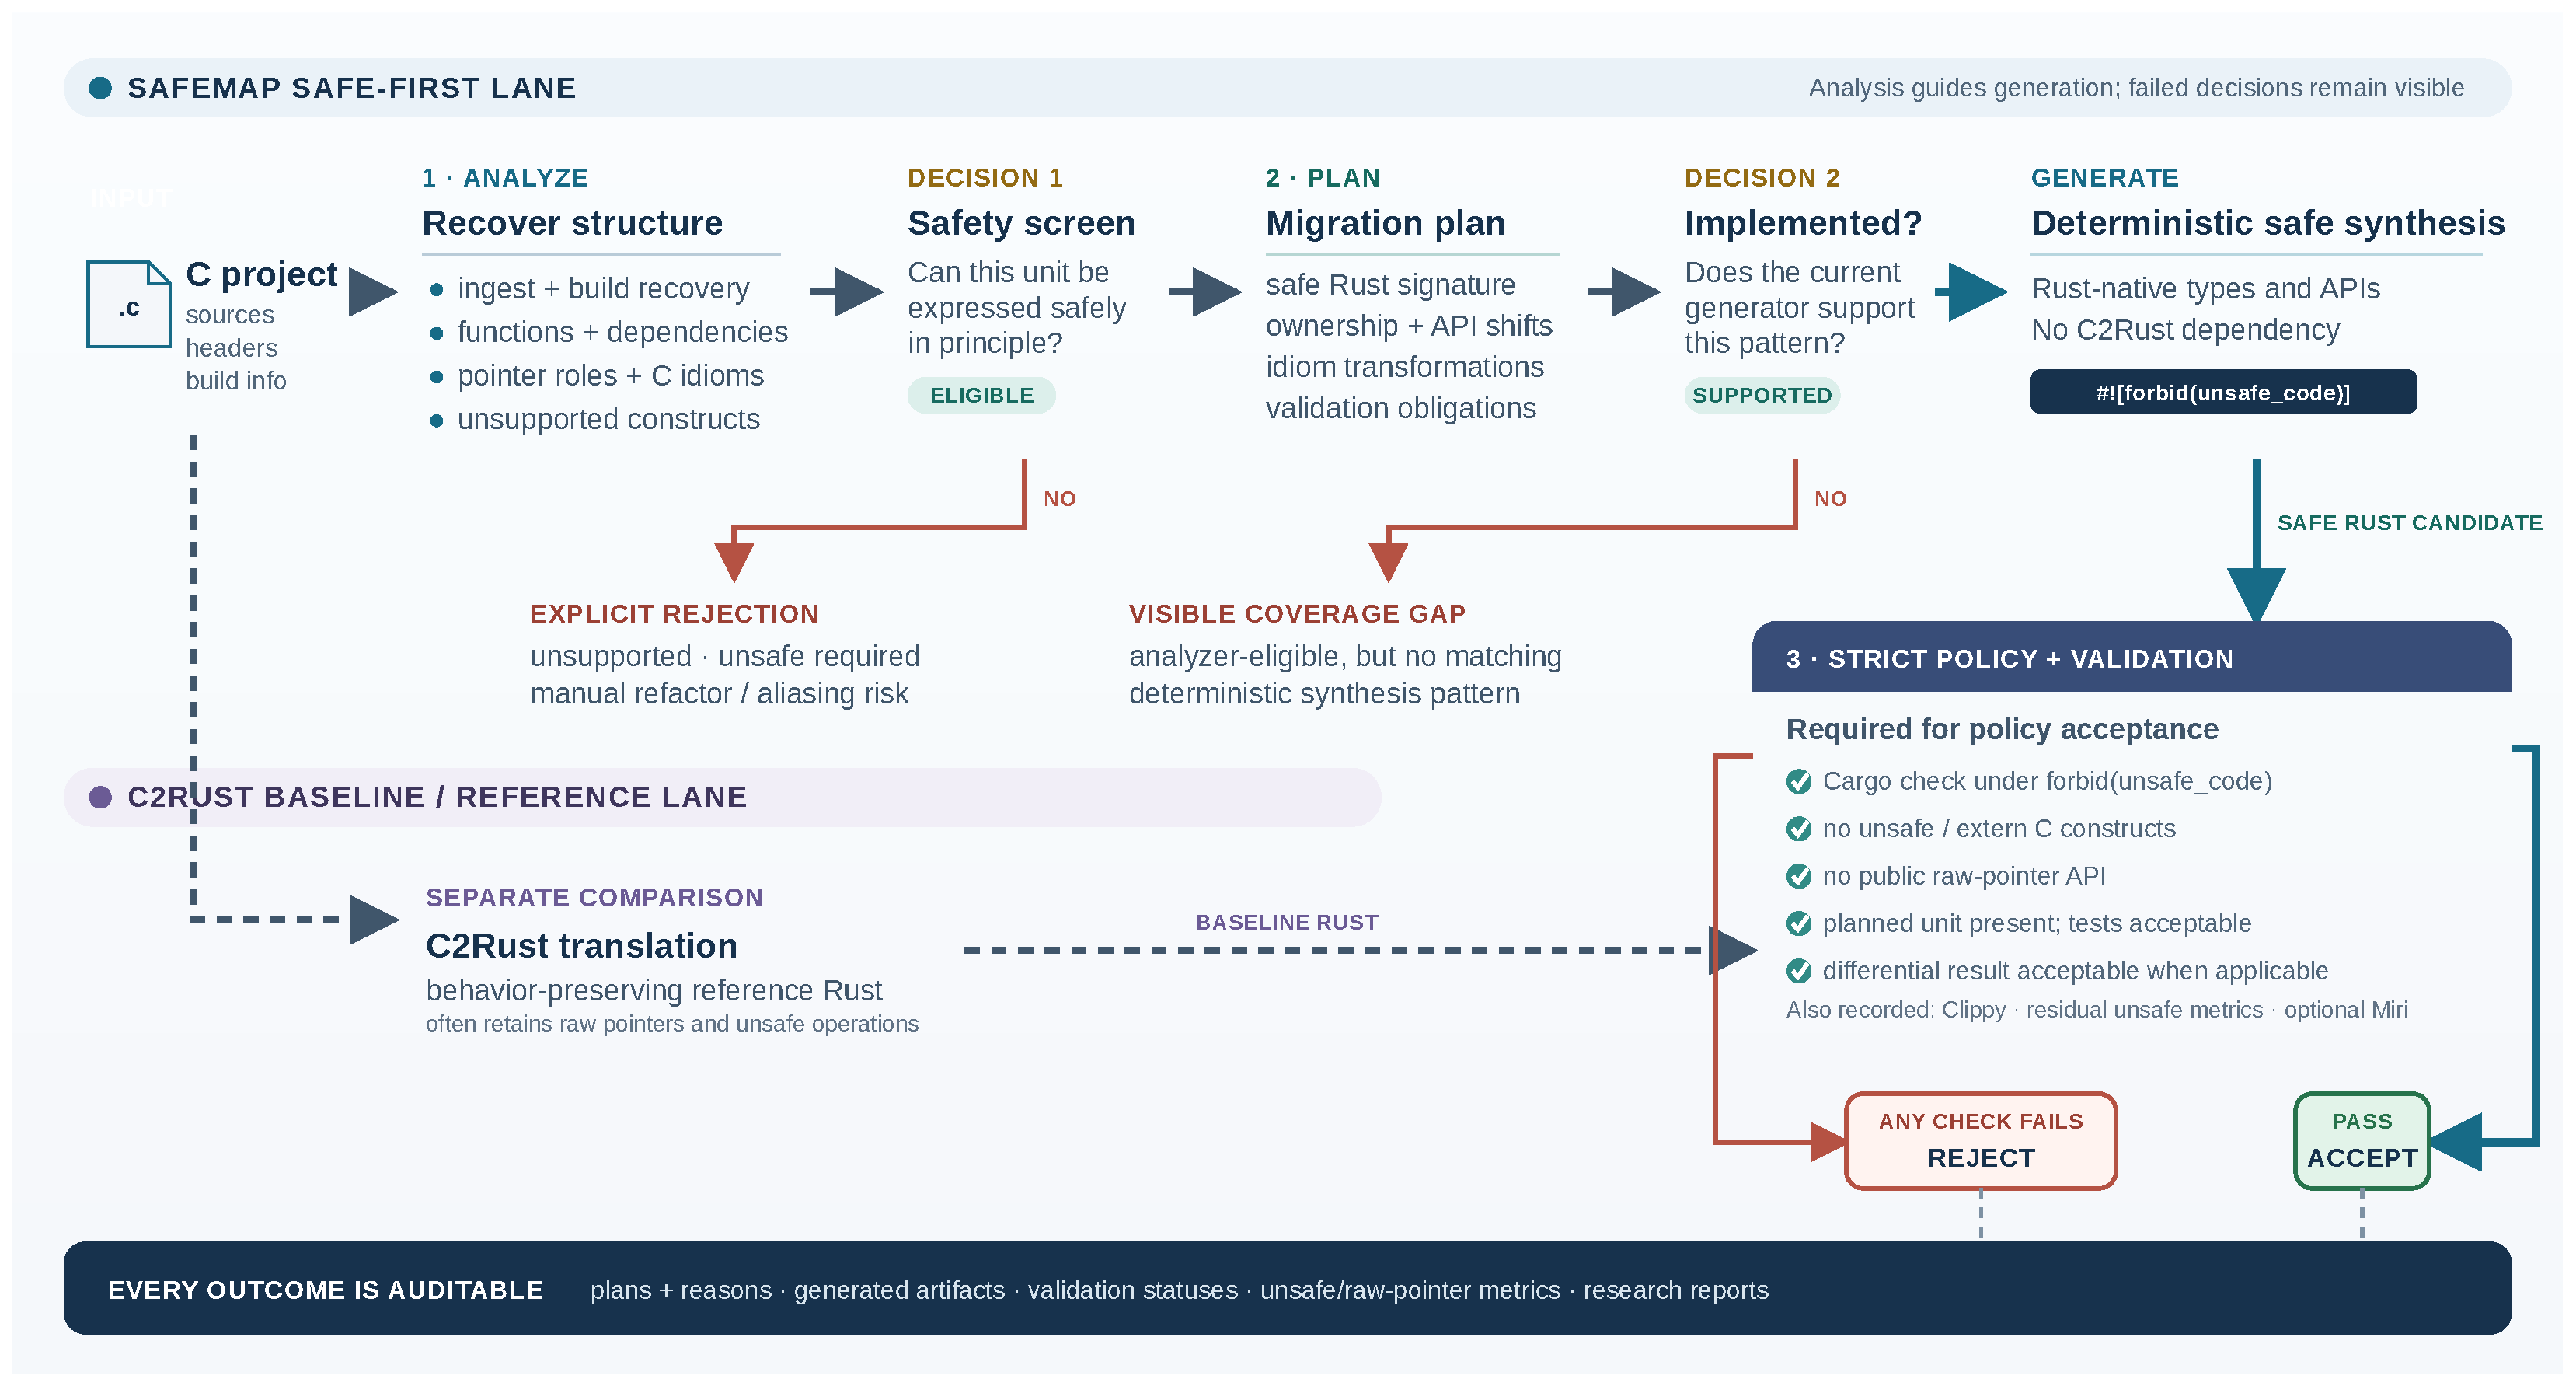
\includegraphics[width=\textwidth]{figures/Fig1}
  \caption{\tool conversion and acceptance pipeline. Static analysis records
  eligibility separately from synthesis support. Where no deterministic rule
  matches a planned unit, the generation step issues a plan-guided LLM request
  with compiler-feedback repair (not drawn). C2Rust runs in a separate
  reference lane. The same policy applies to every output, and reports retain
  refused units, failed checks, and their reasons}
  \label{fig:safemap-pipeline}
\end{figure*}

\subsection{Deterministic rules and plan-guided synthesis}

Deterministic rules cover scalar expressions, boolean and bit-reversal
idioms, pointer-length and fixed-size arrays, scalar structs and field access,
dependency-ordered internal calls, output parameters, return-code plus
output-parameter to \texttt{Result}, nullable pointers, reductions, simple C
string lengths, and simple allocation-to-\texttt{Vec} and \texttt{Box}
patterns. A rule that renders a single expression applies only when the whole
function body is that statement and the expression references only
parameters and called functions.

When no rule applies, \tool sends the LLM the C function, the macros, enums,
and constant tables it references, the Rust definitions of the planned
structs, the signatures of already-accepted callees, the analysis facts, and
the migration plan, and asks for exactly the planned signature. The response is
admitted only if it passes the policy check and compiles with the units
already admitted; otherwise the compiler diagnostics are returned for up to
three repairs.

Consider the LLVM development helper below. libclang finds two indexed
pointers paired with \texttt{n} and no writes, so the plan maps each
pointer-length pair to a shared slice, and the \texttt{slice\_dot\_product}
rule applies:
\begin{lstlisting}[language=C,basicstyle=\ttfamily\scriptsize]
double loop(float *x, float *y, long n) {
  double acc = 0.0;
  for (long i=0; i<n; ++i) acc += (double)x[i] * (double)y[i];
  return acc;
}
\end{lstlisting}
\begin{lstlisting}[basicstyle=\ttfamily\scriptsize]
pub fn r#loop(x: &[f32], y: &[f32]) -> f64 {
  x.iter().zip(y.iter()).map(|(&a,&b)| (a as f64)*(b as f64))
   .fold(0.0_f64, |s,v| s + v)
}
\end{lstlisting}
The initial value \texttt{+0.0} is necessary: differential testing showed that
\texttt{sum()} can disagree with C on the sign of zero.

\subsection{Per-unit differential harness}
\label{sec:harness}

For each admitted unit, \tool generates inputs from a fixed seed, including
integer literals mined from the C body and their neighbors, and embeds the same
literal tables in a C harness and a Rust harness. Slice and array arguments
are exact-size heap buffers, so an out-of-bounds read in C is caught by ASan
rather than masked. The C harness includes the original translation unit and
runs under ASan and UBSan with \texttt{-fno-sanitize-recover=all}; the Rust
harness is built with overflow checks. Return values and every value written
through a mutable parameter are compared exactly (floating point by bit
pattern, strings byte by byte). An input on which the C oracle stops with a
sanitizer report has no defined behavior and is excluded and counted. A
defined C \texttt{abort} or \texttt{exit} must be matched by a Rust panic. A
unit needs at least 50\% defined inputs; otherwise it is recorded as
\texttt{c\_oracle\_undefined\_behavior}.

\subsection{Baselines}

\emph{Rules only} runs the same pipeline without the LLM. \emph{Raw C2Rust}
translates each project in a pinned container (C2Rust 0.22.1, LLVM 14) and is
measured under the same policy. The \emph{one-shot LLM} baseline is given the
same task as \tool in a single request: the project's C sources and headers,
the planned public signatures (C names kept), and the Rust struct definitions
those signatures use, with private helpers allowed. It receives none of
\tool's analysis facts, plans, rules, or repair. Its output is scored with the
same per-unit harness after making top-level functions public. A baseline
that is not told the interfaces cannot be tested through them, so giving them
isolates what \tool adds beyond interface planning; the contribution of
interface planning itself is measured by ablation.

\section{Evaluation methodology}

\subsection{Earlier evaluation}
\label{sec:history}

A first frozen evaluation (protocol v1) ran \tool on inih, cJSON, and libcsv
and accepted 0 of 142 units. Every one of six defects independently forced
that result: the signature planner mapped C types incorrectly; rules fired on
partial matches and emitted template code; struct definitions in headers were
not collected; acceptance was all-or-nothing per project; the C2Rust setup
shadowed libc headers; and the harness covered only scalar shapes. Because the
v1 corpus was inspected while diagnosing these defects, it is used here only
as development data, and the corrected system was evaluated on newly selected
libraries under a new protocol.

\subsection{Protocol}

The v2 protocol fixed the selection rule, configurations, model, acceptance
policy, and reporting before any \tool execution on the held-out corpus. A
library qualifies if it is a public Git repository with an OSI-approved
license, its production code is one \texttt{.c} file plus headers that
compiles against libc alone, the file has 150--3,500 lines, and it was not
used during development. All functions in the file are retained. The protocol
and corpus manifest were sealed and the implementation frozen at commit
\texttt{62cf430} before the corpus was materialized; a materialization script
refuses to run on any other commit. The full test suite passed at the freeze.

Four libraries were selected first: parson, sds, tinyexpr, and microtar.
After their results were seen, we judged four libraries too few and added six
more by the same rule (amendment 1): json-parser, tiny-regex-c, tiny-AES-c,
semver.c, argparse, and printf. Nine candidates qualified in a fresh screen;
six were chosen for domain diversity before any \tool execution on them. The
implementation, configuration, and modes were unchanged. We report the two
rounds separately and pooled. Table~\ref{tab:v2-corpus} characterizes the
corpus.

% Generated by scripts/generate_v2_manuscript_tables.py; do not edit.
\begin{table}[t]
\centering
\caption{Held-out corpus: ten libraries from two selection rounds. LOC: lines of code; Ptr. params: pointer parameters; Complexity: total cyclomatic complexity.}
\label{tab:v2-corpus}
\scriptsize
\begin{tabular}{llrrrrr}
\toprule
Library & Round & C LOC & Functions & Units & Ptr. params & Complexity \\
\midrule
microtar & Original & 376 & 25 & 25 & 39 & 68 \\
parson & Original & 2494 & 144 & 138 & 206 & 633 \\
sds & Original & 1328 & 45 & 45 & 27 & 292 \\
tinyexpr & Original & 1025 & 48 & 37 & 28 & 306 \\
\midrule
argparse & Extension & 395 & 13 & 13 & 27 & 101 \\
json-parser & Extension & 1186 & 10 & 10 & 15 & 227 \\
printf & Extension & 914 & 34 & 20 & 27 & 296 \\
semver & Extension & 638 & 33 & 33 & 29 & 127 \\
tiny-AES-c & Extension & 572 & 20 & 20 & 33 & 47 \\
tiny-regex-c & Extension & 528 & 18 & 15 & 23 & 126 \\
\midrule
Total &  & 9456 & 390 & 356 & 454 & 2223 \\
\bottomrule
\end{tabular}
\end{table}


\subsection{Configuration}

All LLM configurations, \tool and baseline alike, use Google's
\texttt{gemini-3.5-flash-lite} at temperature zero through its
OpenAI-compatible API, with at most three repairs per unit, 1,000 generated
inputs per unit, and seed 20260728. The evaluation used the provider's free
tier. A request still refused after the client's retries stops the run rather
than being scored as a failure; the run resumes after the quota resets, reusing
every finished (project, configuration) result. Because LLM output can vary
even at temperature zero, the LLM configurations were run three times on every
held-out library with identical inputs; the first run is the primary result.
Tool versions: rustc and Clippy 1.99.1, Clang 23.1.3; C2Rust 0.22.1 with LLVM
14 in a pinned container.

\subsection{Development data}

Development data comprises 40 authored microbenchmarks, six authored modules,
ten LLVM test-suite programs pinned at commit \texttt{6cdc54e}
\cite{llvmtestsuite}, and the three v1 libraries. Their results informed the
corrections, so they are not evidence of generalization. The component
ablations are run on the v1 libraries with the frozen implementation and are
reported as development data, which keeps the held-out LLM run within the
provider's quota.

\subsection{Mutation analysis}

To test whether the per-unit check rejects wrong code, we applied
single-operator mutations (relational, arithmetic, logical, boolean, and
integer-literal changes) to every accepted function of \tool's held-out runs and
of its v1-library run, kept the mutants that compile, and re-ran each unit's
differential test with 300 inputs.

\section{Results}
\label{sec:results}

\subsection{RQ1: Accepted units}

Table~\ref{tab:v2-cascade} follows each held-out unit through the pipeline.
In the first run, of 356 units, the screen marked 183 as candidates, \tool generated Rust for 47,
and accepted 16 (4.5\% of all units; 8.7\% of candidates). The original four
libraries contributed 7 accepted units and the extension 9. Accepted units
are small leaf functions: a string hash, hexadecimal and UTF-8 helpers,
rounding, error strings, version-string checks, regular-expression character
classes, and the AES \texttt{xtime} step.

% Generated by scripts/generate_v2_manuscript_tables.py; do not edit.
\begin{table}[t]
\centering
\caption{\tool (guided) outcome cascade per library (first run, per-unit Clippy; sealed result in parentheses where it differs). \emph{Crate}: the unit passed \texttt{cargo check} and tests, and Clippy found no error in it or in its callees.}
\label{tab:v2-cascade}
\scriptsize
\begin{tabular}{lrrrrrr}
\toprule
Library & Units & Candidate & Generated & Crate & Policy & Accepted \\
\midrule
microtar & 25 & 3 & 2 & 2 & 2 & 2 \\
parson & 138 & 72 & 4 & 4 & 4 & 3 \\
sds & 45 & 30 & 4 & 4 & 4 & 2 \\
tinyexpr & 37 & 32 & 24 & 22 (0) & 22 (0) & 21 (0) \\
\midrule
argparse & 13 & 0 & 0 & 0 & 0 & 0 \\
json-parser & 10 & 3 & 2 & 2 & 2 & 1 \\
printf & 20 & 18 & 0 & 0 & 0 & 0 \\
semver & 33 & 17 & 4 & 4 & 4 & 3 \\
tiny-AES-c & 20 & 1 & 1 & 1 & 1 & 1 \\
tiny-regex-c & 15 & 7 & 6 & 6 & 6 & 4 \\
\midrule
Total & 356 & 183 & 47 & 45 (23) & 45 (23) & 37 (16) \\
\bottomrule
\end{tabular}
\end{table}


Of the 31 generated units not accepted, 24 are from tinyexpr. They compiled,
but the crate failed Clippy: two translated constants, \texttt{pi} and
\texttt{e}, keep C's literal digits, which Clippy's default-deny
\texttt{approx\_constant} lint rejects. Because Clippy runs once per crate,
this rejected every unit in the crate. We report the outcome as frozen; it is
a limitation of crate-level checks within a per-unit policy
(Section~\ref{sec:threats}).

\subsection{RQ2: Why units are not accepted}

Table~\ref{tab:v2-refusals} lists the recorded reasons. Most units never
reach translation. 159 functions require manual refactoring, mainly because
they read or write mutable global state, perform I/O, or follow allocation
protocols that cross function boundaries. 116 use a C type for which the
planner finds no safe, testable interface: in parson and sds the central types
(\texttt{JSON\_Value *}, \texttt{sds}) are opaque handles or point into the
middle of an allocation, and \texttt{void *} and \texttt{char **} parameters
are common. 36 require unsafe operations such as pointer arithmetic beyond a
known length or casts between pointer types. Only a small fraction of losses
occur after translation: 3 differential-test failures, and 4 units whose C
oracle had undefined behavior on most generated inputs. Two of these show a
limit of signature-level planning: sds's \texttt{sdsll2str} writes up to 21
bytes into a caller buffer, a requirement its signature does not express, so
every generated buffer overflowed. The other two overflow signed arithmetic on
most inputs.

% Generated by scripts/generate_v2_manuscript_tables.py; do not edit.
\begin{table}[t]
\centering
\caption{Recorded reasons for functions not accepted by \tool (guided), all ten held-out libraries (first run).}
\label{tab:v2-refusals}
\scriptsize
\begin{tabular}{lr}
\toprule
Reason & Functions \\
\midrule
Manual refactor (global state, I/O, allocation protocols) & 159 \\
No safe, testable interface for a C type & 116 \\
Requires unsafe (raw memory, casts) & 36 \\
Crate-level Clippy check failed & 24 \\
Unsupported construct (union, function pointer, asm) & 12 \\
C undefined on most test inputs & 4 \\
Differential test failed & 3 \\
Callee not translated & 3 \\
No synthesis plan & 3 \\
\bottomrule
\end{tabular}
\end{table}


\subsection{RQ3: Baselines}

Table~\ref{tab:v2-baselines} compares the configurations. \tool accepted 16
units in the first run, the one-shot LLM 9, rules alone 1, and C2Rust none.
Over three runs the ranges overlap (Table~\ref{tab:v2-repeats}), so we do not
claim that \tool outperforms the one-shot baseline. \tool used 40 LLM
requests and the one-shot baseline 8 (one per library with planned
interfaces). The one-shot baseline benefits from \tool's interface planning:
without the planned signatures, its output could not be tested function by
function. Raw C2Rust output compiled for seven of ten libraries; for parson,
sds, and printf it failed on the pinned toolchain because its
\texttt{va\_list} handling and packed-struct field references are rejected by
current rustc. Where it compiled, it contained unsafe code and raw-pointer
interfaces throughout, so no unit met the policy.

% Generated by scripts/generate_v2_manuscript_tables.py; do not edit.
\begin{table}[t]
\centering
\caption{Accepted units per configuration on the held-out libraries (first run). One-shot: given the planned signatures; plain: C sources only (amendment 2). LLM calls: guided / one-shot. $^\dagger$C2Rust output did not compile.}
\label{tab:v2-baselines}
\scriptsize
\begin{tabular}{lrrrrrrr}
\toprule
Library & Units & Guided & One-shot & Plain & Rules & C2Rust & LLM calls \\
\midrule
microtar & 25 & 2 & 1 & 0 & 1 & 0 & 1 / 1 \\
parson & 138 & 3 & 4 & 0 & 0 & 0$^\dagger$ & 4 / 1 \\
sds & 45 & 2 & 0 & 0 & 0 & 0$^\dagger$ & 4 / 1 \\
tinyexpr & 37 & 0 & 0 & 0 & 0 & 0 & 17 / 1 \\
\midrule
argparse & 13 & 0 & 0 & 0 & 0 & 0 & 0 / 0 \\
json-parser & 10 & 1 & 1 & 0 & 0 & 0 & 2 / 1 \\
printf & 20 & 0 & 0 & 0 & 0 & 0$^\dagger$ & 0 / 0 \\
semver & 33 & 3 & 0 & 1 & 0 & 0 & 5 / 1 \\
tiny-AES-c & 20 & 1 & 1 & 0 & 0 & 0 & 1 / 1 \\
tiny-regex-c & 15 & 4 & 2 & 0 & 0 & 0 & 6 / 1 \\
\midrule
Total & 356 & 16 & 9 & 1 & 1 & 0 & 40 / 8 \\
\bottomrule
\end{tabular}
\end{table}


Development data show the same pattern (Table~\ref{tab:v2-development}): on
the v1 libraries the two accepted 22 and 21 units. Only on the authored
microbenchmarks, which the rules were written for, is \tool clearly ahead
(72 of 81 units against 35).

% Generated by scripts/generate_v2_manuscript_tables.py; do not edit.
\begin{table}[t]
\centering
\caption{Development data: accepted units per configuration.}
\label{tab:v2-development}
\scriptsize
\begin{tabular}{lrrrrr}
\toprule
Corpus & Units & Guided & One-shot LLM & Rules only & C2Rust \\
\midrule
Microbenchmarks & 81 & 72 & 35 & 35 & 0 \\
Authored modules & 25 & 24 & 18 & 18 & 0 \\
LLVM programs & 32 & 10 & 8 & 6 & 0 \\
v1 libraries & 142 & 22 & 21 & 0 & 0 \\
\bottomrule
\end{tabular}
\end{table}


\subsection{RQ4: Component ablations}

Table~\ref{tab:v2-ablations} reports the ablations on the v1 libraries.
The full system accepted 22 of 142 units. Removing safe-signature planning
reduced this to 2, while raising LLM requests from 23 to 126, because the model must
then invent interfaces that rarely compile with their callers. Removing idiom
plans reduced acceptance to 3. Withholding analysis facts and plans from the
prompt or removing compiler-feedback repair changed nothing (22), removing
dependency grouping lost one unit (21), and removing pointer roles lost one
(21). The planning that determines \emph{what} interface each
function gets, rather than the guidance given to the LLM, accounts for the
accepted translations.

% Generated by scripts/generate_v2_manuscript_tables.py; do not edit.
\begin{table}[t]
\centering
\caption{Component ablations on the v1 libraries (development data): accepted / all units.}
\label{tab:v2-ablations}
\scriptsize
\begin{tabular}{lrrrr}
\toprule
Configuration & cJSON & inih & libcsv & LLM calls \\
\midrule
Full system & 15/109 & 1/10 & 6/23 & 23 \\
Facts and plan withheld from prompt & 15/109 & 1/10 & 6/23 & 22 \\
Without pointer roles & 15/109 & 0/10 & 6/23 & 23 \\
Without safe signatures & 2/109 & 0/10 & 0/23 & 126 \\
Without dependency grouping & 14/113 & 1/10 & 6/23 & 21 \\
Without idiom plans & 3/109 & 0/10 & 0/23 & 3 \\
Without compiler-feedback repair & 15/109 & 1/10 & 6/23 & 22 \\
\bottomrule
\end{tabular}
\end{table}


\subsection{RQ5: Reliability of acceptance}

\textbf{Mutation analysis.} Of 304 compiling mutants of accepted functions
(all ten held-out libraries and the v1 libraries), the per-unit check rejected
270 (88.8\%). Survivors concentrate in functions whose behavior depends on
narrow input ranges: six of the 34 are in sds's hexadecimal-digit converter whose branches are reached only by the few
generated inputs that are hexadecimal characters. Some survivors may be
equivalent mutants; we did not classify them.

\textbf{Repeated runs.} Table~\ref{tab:v2-repeats} reports accepted units in
three runs of the LLM configurations with identical inputs. \tool accepted 16,
15, and 12 units, the one-shot baseline 9, 15, and 14. Eight of the ten
libraries gave the same \tool result in every run. Most of the variation comes
from semver: in one run of each configuration, one generated function failed a
crate-level check and so rejected all four planned units of that crate, the
same mechanism as tinyexpr. The accepted sets are therefore stable at the
function level but sensitive to crate-level failures.

% Generated by scripts/generate_v2_manuscript_tables.py; do not edit.
\begin{table}[t]
\centering
\caption{Accepted units across repeated LLM runs (identical inputs and configuration), with per-unit Clippy; sealed result in parentheses where it differs. One-shot: given the planned signatures; plain: C sources only.}
\label{tab:v2-repeats}
\scriptsize
\begin{tabular}{lrrrr}
\toprule
Run & Libraries & Guided & One-shot & Plain \\
\midrule
Run 1 & 10 & 37 (16) & 28 (9) & 1 \\
Run 2 & 10 & 36 (15) & 31 (15) & 1 \\
Run 3 & 10 & 36 (12) & 30 (14) & 2 \\
\bottomrule
\end{tabular}
\end{table}


\section{Discussion}

\textbf{Coverage is the limiting factor.} The per-function acceptance check is
feasible on production C and rejects most wrong code, but few functions reach
it. Table~\ref{tab:v2-refusals} is the main finding: the obstacles are global
state, opaque and aliasing pointer types, and raw memory manipulation. These
are API design questions that a function-local translator cannot answer
alone; a migration would need to change the library's interface, for example
by turning global state into an explicit context or an \texttt{sds} string
into an owned type, before \tool's checks apply.

\textbf{Interfaces matter more than prompts.} Given the planned interfaces, a
single LLM request performs within the run-to-run range of \tool's guided loop;
without them, the guided loop collapses (2 of 142 units). Withholding analysis
facts from the prompt changed nothing on the v1 libraries. This suggests that LLM translators benefit most from being
told the target interface, which is consistent with CRUST-Bench's use of
hand-written interfaces \cite{khatry2025crustbench}.

\textbf{Refusal as output.} Every refused unit carries a reason and the plan
that produced it. For a migration team this identifies which functions can be
migrated mechanically and which need design work.

\section{Threats to validity}
\label{sec:threats}

\textbf{Sample.} Ten small libraries with one production file each do not
represent large applications or multi-file projects. The extension was decided
after the first four results were seen; it used the same rule and frozen code,
and we report both rounds separately.

\textbf{Model and variance.} One low-cost model was used, and three runs
are too few to estimate run-to-run variance precisely; the guided and one-shot
ranges overlap, so their difference is not established. A stronger model may translate
more of the planned units, although it cannot change the units refused before
translation, which are most of the losses.

\textbf{Oracle.} Differential testing on generated inputs is evidence, not
proof. Mutation analysis shows that 11.2\% of compiling mutants survive,
mainly where inputs rarely reach a branch. Excluding inputs with undefined C
behavior removes inputs the sanitizers detect, not all undefined behavior.

\textbf{Crate-level checks.} Clippy runs on the whole crate, so one lint error
rejects every unit in it (tinyexpr). This makes the reported numbers
conservative.

\textbf{No eligibility labels.} We did not collect independent labels of
which functions could be migrated safely, so we make no claim about the
precision or recall of the screen; refusals are reported as recorded.

\textbf{Toolchain.} C2Rust 0.22.1's output does not compile with the pinned
nightly on three libraries; another toolchain might compile it, but it would
still use unsafe code and fail the policy.

\textbf{Development data.} The development corpora and the v1 libraries
shaped the implementation; results on them are not evidence of
generalization, and the ablations are run on them.

\section{Conclusion}

\tool translates C functions to safe Rust only when it finds a safe interface
and accepts them only when they match the original C under sanitizers. On ten
held-out libraries it accepted 12--16 of 356 units across three runs, against
9--15 for a one-shot LLM given the same planned interfaces, 1 for its rules
alone, and 0 for raw C2Rust. The interface planning, not the LLM guidance, is
what makes these translations possible to produce and check. Most units
are refused before translation because of global state, opaque or aliasing
pointer types, or unsafe memory operations. Per-function, oracle-checked
migration is therefore feasible but narrow: its reach is set by how much of a
C library's interface already has a safe Rust counterpart. Future work should
plan such interface changes explicitly, generate inputs that target narrow
branches, and run lint checks per unit.

\section*{Statements and Declarations}

\subsection*{Funding}
No funding was received for conducting this study or preparing this manuscript.

\subsection*{Competing interests}
The authors declare no competing financial or non-financial interests relevant
to the content of this article.

\subsection*{Data availability}
The source code, evaluation protocol, corpus manifests, configuration, frozen
implementation record, raw results, and scripts that generate every table are
available in the SafeMAP repository
(\url{https://github.com/jscyril/SafeMAP}); the implementation evaluated here
is commit \texttt{62cf430}. The result rows of every run are in
\texttt{reports/publication/v2}, and
\texttt{scripts/generate\_v2\_manuscript\_tables.py} regenerates every table
from them. The held-out libraries are public repositories
pinned to the revisions recorded in the manifests.

\subsection*{Ethics approval}
Not applicable. The study involved no human participants.

\subsection*{Use of generative AI}
Generative AI tools were used in this work. ChatGPT assisted with generating
the synthetic development benchmarks and with language refinement. Claude
assisted with implementing and testing the software, writing the evaluation
scripts, and drafting and revising the manuscript. The evaluated pipeline
itself calls Gemini as described in the paper. The authors reviewed and
validated all AI-assisted code, data, and text, and remain responsible for the
accuracy, originality, and integrity of the manuscript.

\subsection*{Author contributions}
Jacob Sebastian Cyril: conceptualization, methodology, software,
investigation, formal analysis, visualization, and writing---original draft.
Benita Jose Chalissery: research guidance and manuscript review. NewBegin M:
supervision and manuscript review. All authors approved the final manuscript.

{\def\bibfont{\footnotesize}\bibliography{references}}

\end{document}
